%\chapter{Derivation of two-dimensional PDEs for water waves at random intermediate depths}
%\chapter{Derivation of a two-dimensional PDE for water waves at varying water depths}
\chapter{A two-dimensional PDE for water waves at varying water depths}
\label{chap:pde_derivation}

In this appendix, I will present a new \idx{two-dimensional} \index{dimensionality!two|see{two-dimensional}} \PDE in the \idxs{spatial}{domain}, describing the \qidxs{time evolution of}{surface waves} for intermediate, mildly varying water depths. The equation could efficiently be solved with a \idx{time complexity} of $O(N)$\indexs{big O}{notation} per \idx{time step}, where $N$ is the number of \idxsp{surface}{grid point}{s}, using the \CFMM \citep{White1994}. It has not been solved numerically so its behavior is unknown.

The equation is derived from the \idxs{dispersion}{relation} that is obtained in \idxs{Airy wave}{theory}\index{wave theory!Airy|see{Airy wave theory}}, namely:

\begin{equation} \label{eq:dispersion_again}
\omega^2(k) \,=\, \left(g\,+\,\frac{\gamma}{\rho}\,k^2\right)\,k\,\tanh(k\,h),
\end{equation}

where $\omega$ is the \idxs{angular}{frequency} of one \idxs{wave}{component}, $k$ is the \idx{wavenumber} of the component, $g$ is the \idxs{gravitational}{acceleration}, $h$ is the \idxs{water}{depth} and $\gamma$ is the \idxs{surface}{tension}. Since this equation describes waves of a single \idx{wavelength}, we can assume that the \idxs{free surface}{elevation} for one wave component can be described by

\begin{equation} \label{eq:component}
\eta(\vec{r},\,t) \,=\, A\,e^{i(\vec{k}\cdot\vec{r}\,-\,\omega\,t)},
\end{equation}

where $\eta$ is the so far \idx{complex-valued} free surface elevation, $A$ is the \idxs{wave}{amplitude} which can be any \idxs{complex}{number} and $\vec{k}$ is the wave vector. We make the observation that $k$ and $\vec{k}$ are related to each other by

\begin{equation} \label{eq:kvectok}
k \,=\, \left|\vec{k}\right|.
\end{equation}

Although \eqref{eq:component} describes the time evolution of all wave components, it includes variables from the \idxs{frequency}{domain} ($\vec{k}$ and $\omega$ --- note that $k$ depends on $\vec{k}$ according to \eqref{eq:kvectok}), which are not available when working purely in the spatial domain. Furthermore, the equation is indirectly dependent on $h$ and assumes that this variable has the same value on all locations, which may not be the case. We therefore need a way to express the time evolution of the free surface which does not use frequency domain variables and is robust even for varying water depths.

By \idxe{differentiation!in time}{differentiating} \eqref{eq:component} in time, we obtain

\begin{equation}
\frac{\partial\eta(\vec{r},\,t)}{\partial t} \,=\, -i\,\omega\,A\,e^{i(\vec{k}\cdot\vec{r}\,-\,\omega\,t)},
\end{equation}

where $i$ is the \idxs{imaginary}{unit}. The equation can be rewritten as

\begin{equation}
\frac{\partial}{\partial t}\eta(\vec{r},\,t) \,=\, -i\,\omega\,\eta(\vec{r},\,t).
\end{equation}

In a manner inspired by the derivation of the \idxs{Schrödinger}{equation} \citep{Bransden2000}, let's define the \idxs{scalar}{operator}

\begin{equation} \label{eq:opomega}
\sop{\omega} \,=\, i\frac{\partial}{\partial t}
\end{equation}

and we see that

\begin{equation} \label{eq:opomegaaction}
\sop{\omega}\,\eta \,=\, \omega\,\eta
\end{equation}

for a wave component described by \eqref{eq:component}. By taking the \idx{gradient} of \eqref{eq:component}, we obtain

\begin{equation}
\nabla\eta(\vec{r},\,t) \,=\, i\,\vec{k}\,A\,e^{i(\vec{k}\cdot\vec{r}\,-\,\omega\,t)}
\end{equation}

which can be written as

\begin{equation}
\nabla\eta(\vec{r},\,t) \,=\, i\,\vec{k}\,\eta(\vec{r},\,t).
\end{equation}

Let's define the \idxse{vector}{operator}{vector} and \idxsp{scalar}{operator}{s}

\begin{samepage}
\begin{equation} \label{eq:opkvec}
\vop{k} \,=\, -i\,\nabla
\end{equation}

\begin{equation} \label{eq:opk2}
\sop{k^2} \,=\, \vop{k}^2 \,=\, -\nabla^2
\end{equation}
\end{samepage}

and we see that 

\begin{samepage}
\begin{equation} \label{eq:opkvec1action}
\phantom{and}\quad\vop{k}\,\eta \,=\, \vec{k}\,\eta,\quad\text{and}
%\vop{k}\,\eta \,=\, \vec{k}\,\eta,
\end{equation}

\begin{equation} \label{eq:opk2action}
\sop{k^2}\,\eta \,=\, k^2\,\eta
\end{equation}
\end{samepage}

for a wave component described by \eqref{eq:component}. By multiplying both sides of \eqref{eq:dispersion_again} with $\eta$, we obtain

\begin{equation}
\omega^2\,\eta \,=\, \left(g\,+\,\frac{\gamma}{\rho}\,k^2\right)\,k\,\tanh(k\,h)\,\eta
\end{equation}

which can be rewritten as

\begin{equation} \label{eq:diffeqbad}
\sop{\omega}^2\,\eta \,=\, \left(g\,+\,\frac{\gamma}{\rho}\,\sop{k^2}\right)\,k\,\tanh(k\,h)\,\eta.
\end{equation}

We now have an equation almost free from $\vec{k}$ and $\omega$. However, the factor $k\,\tanh(k\,h)$ persists and is difficult to turn into an operator free from $\vec{k}$. One solution is to turn this factor into a \idxs{convolution}{filter} which works by calculating the \idx{convolution} between the operand and a \idxs{convolution}{kernel}. However, the kernel proves to be difficult to obtain due to the asymptotically increasing value of $k\,\tanh(k\,h)$ as $k\rightarrow\infty$. A possibility is to rewrite \eqref{eq:diffeqbad} into

\begin{equation} \label{eq:diffeqbetter}
\sop{\omega}^2\,\eta \,=\, h\,\left(g\,+\,\frac{\gamma}{\rho}\,\sop{k^2}\right)\,\sop{k^2}\,\fdfunc{K}(\vec{k}\,h)\,\eta,
\end{equation}

where

\begin{equation} \label{eq:transkernelofxivec}
\fdfunc{K}(\vec{\xi}) \,=\, \begin{cases}
1                                                  , & \quad \vec{\xi} = \vec{0} \\[.5em]
\displaystyle\frac{\tanh(|\vec{\xi}|)}{|\vec{\xi}|}, & \quad \vec{\xi} \neq \vec{0}
\end{cases}\ ,
\end{equation}

a $\fdfunc{\ }$ denotes a function or a variable in the frequency domain and $\vec{\xi}$ is a \idxs{dimensionless}{vector}\index{unitless!see{dimensionless}} in the frequency domain, and turn $\fdfunc{K}(\vec{\xi})$ into a convolution filter. The effect of a \idxs{scalar}{operator} $\sop{C}$ applying the filter on a function described by \eqref{eq:component} would be

\begin{equation} \label{eq:opceffect}
\sop{C}\,\eta(\vec{r},\,t) \,=\, \fdfunc{K}(\vec{k}\,h)\,\eta(\vec{r},\,t)
\end{equation}

and since the operator applies a convolution filter, it can be described by

\begin{equation} \label{eq:opcfconvolution}
\sop{C}\,\eta(\vec{r},\,t) \,=\, \{f\,*\,\eta\}(\vec{r},\,t),
\end{equation}

where $f$ is the \idxs{convolution}{kernel}. With this new operator, \eqref{eq:diffeqbetter} can be rewritten further into

\begin{equation} \label{eq:diffeqspatial}
\sop{\omega}^2\,\eta \,=\, h\,\left(g\,+\,\frac{\gamma}{\rho}\,\sop{k^2}\right)\,\sop{k^2}\,\sop{C}\,\eta.
\end{equation}

which is a \PDE completely free from variables in the frequency domain. Combining \eqref{eq:opceffect} and \eqref{eq:opcfconvolution} yields

\begin{equation} \label{eq:fconvolutioneffect}
\{f\,*\,\eta\}(\vec{r},\,t) \,=\, \fdfunc{K}(\vec{k}\,h)\,\eta(\vec{r},\,t).
\end{equation}

The \idx{convolution theorem} states that

\begin{equation} \label{eq:convolutiontheorem}
\mathcal{F}\{f\,*\,g\} \,=\, \mathcal{F}\{f\}\,\cdot\,\mathcal{F}\{g\},
\end{equation}

where $\mathcal{F}$ denotes the \idxs{non-unitary}{Fourier transform} and $\cdot$ denotes point-wise multiplication. By Fourier transforming \eqref{eq:fconvolutioneffect} using this theorem, we obtain

\begin{equation}
\mathcal{F}\{f\}(\vec{k})\ \mathcal{F}\{\eta\}(\vec{k},\,t) \,=\, \fdfunc{K}(\vec{k}\,h)\ \mathcal{F}\{\eta\}(\vec{k},\,t)
\end{equation}

which can be rewritten as

\begin{equation} \label{eq:ffourier}
\mathcal{F}\{f\}(\vec{k}) \,=\, \fdfunc{K}(\vec{k}\,h)
\end{equation}

by canceling out $\mathcal{F}\{\eta\}(\vec{k},\,t)$ on both sides. For scaling of a function with a real, non-zero number $a$, the non-unitary Fourier transform has the following property:

\begin{equation} \label{eq:fourierscaling}
\mathcal{F}\{h\}(\vec{\xi}) \,=\, \frac{1}{|a|^d}\,\mathcal{F}\{f\}\left(\frac{\vec{\xi}}{a}\right)
,\quad
h(\vec{x}) \,=\, f(a\vec{x})\ \forall\ \vec{x},
\end{equation}

where $d$ is the number of dimensions and $\vec{x}$ is a vector with dimensionless values in the \idxs{spatial}{domain}. Let's define the function

\begin{equation} \label{eq:ftokernel}
K(\vec{x}) \,=\, h^2\,f(h\,\vec{x}).
\end{equation}

Since we are working in \idxs{two}{dimensions}, we have $d = 2$, and the scaling property of the non-unitary Fourier transform (\eqref{eq:fourierscaling}) tells us that

\begin{equation}
\mathcal{F}\{K\}(\vec{\xi}) \,=\, h^2\,\frac{1}{|h|^2}\,\mathcal{F}\{f\}\left(\frac{\vec{\xi}}{h}\right)
\end{equation}

which, by using \eqref{eq:ffourier} can be rewritten as

\begin{equation}
\mathcal{F}\{K\}(\vec{\xi}) \,=\, \fdfunc{K}(\vec{\xi}).
\end{equation}

$K(\vec{x})$ is obtained by \idxse{reverse}{non-unitary Fourier transform}{reverse Fourier transforming} this equation:

\begin{equation} \label{eq:kernelfour2d}
K(\vec{x}) \,=\, \mathcal{F}^{-1}\{\fdfunc{K}(\vec{\xi})\}(\vec{x}) \,=\, \frac{1}{(2\,\pi)^2}\int_{\mathbb{R}^2}\fdfunc{K}(\vec{\xi})\,e^{i\,\vec{\xi}\cdot\vec{x}}\,\opd\vec{\xi}
\end{equation}

where $\mathcal{F}^{-1}$ denotes the \idxs{reverse}{non-unitary Fourier transform}. Although it is very difficult (if not impossible) to obtain the reverse Fourier transform of this function analytically, it is possible to \idxe{approximation}{approximate} it numerically and use the approximation in the convolution filter instead.

With no loss of generality, we can pick a \idxs{polar}{coordinate system}\index{system!polar coordinate|see{polar coordinate system}} $(\xi,\,\theta)$ such that the vector $\vec{x}$ lies on the $\theta = 0$ axis. In that case, \eqref{eq:kernelfour2d} can be rewritten as

\begin{equation}
K(\vec{x}) \,=\, \frac{1}{(2\,\pi)^2}\int_{\xi=0}^\infty\int_{\theta=0}^{2\,\pi}\fdfunc{K}(\xi, \theta)\,e^{i\,\xi\,x\cos\theta}\,\xi\,\opd\theta\,\opd\xi,
\end{equation}

where $\xi = |\vec{\xi}|$ and $\theta$ is the angle between the $\vec{x}$ and $\vec{\xi}$ vectors. By realizing that $\fdfunc{K}$ is circular symmetric, i.e.

\begin{equation}
\fdfunc{K}(\vec{\xi}) \,=\, \fdfunc{K}(\xi),
\end{equation}

and that this leads to that $K$ also is circular symmetric, i.e.

\begin{equation}
K(\vec{x}) \,=\, K(x),
\end{equation}

where $x = |\vec{x}|$, the integral over $\theta$ may be carried out, and the Fourier transform is now written

\begin{equation} \label{eq:fdkerneltokernel}
K(x) \,=\, \frac{1}{2\,\pi}\int_0^\infty\fdfunc{K}(\xi)\,J_0(x\,\xi)\,\xi\,\opd\xi \,=\, \frac{1}{2\,\pi}\,F_0\{\fdfunc{K}\}(x),
\end{equation}

where $J_0$ is the \idxs{zeroth order}{Bessel function of the first kind} and $F_0$ denotes the \idxs{zeroth order}{Hankel transform}, which can be calculated more efficiently than the reverse \idxs{two-dimensional}{Fourier transform}. The corresponding transformation for calculating $\fdfunc{K}$ from $K$ is given by

\begin{equation} \label{eq:kerneltofdkernel}
\fdfunc{K}(\xi) \,=\, 2\,\pi\,F_0\{K\}(\xi).
\end{equation}

In this case, since $K(x)$ was found to vanish very quickly as $x\rightarrow\infty$, it was more efficient to solve \eqref{eq:kerneltofdkernel} by guessing a function $K^*$ for $K$, transforming it according to

\begin{equation} \label{eq:kerneltofdkernelmodified}
\fdfunc{K}^*(\xi) \,=\, 2\,\pi\,F_0\{K^*\}(\xi),
\end{equation}

which is a modified version of \eqref{eq:kerneltofdkernel}, and comparing $\fdfunc{K}^*$ with $\fdfunc{K}$, than to calculate $K$ from \eqref{eq:fdkerneltokernel} directly. A function that was found both to be simple and to have a high visual resemblance with $\fdfunc{K}$ after transformed according to \eqref{eq:kerneltofdkernelmodified} was

\begin{equation} \label{eq:empirical}
K^*(x) \,=\, \frac{1}{2\,\pi\,x\,(1\,+\,x)}\,e^{-x^2/4},
\end{equation}

where $^*$ denotes an \estimate. A comparison between $\fdfunc{K}^*$ when $K^*$ is given by \eqref{eq:empirical} and $\fdfunc{K}$ can be seen in \figref{fig:transformedkernel}. Note that both $K$, $\fdfunc{K}$ and the arguments they take are \idx{dimensionless}. $K$ is therefore the \idxs{dimensionless}{convolution kernel}.

\begin{figure}
    \centering
    \subcaptionbox{\label{fig:transformedkernelcomparison}}[.43\textwidth]{% Title: glps_renderer figure
% Creator: GL2PS 1.3.6, (C) 1999-2011 C. Geuzaine
% For: Octave
% CreationDate: Wed Jun 13 10:06:23 2012
\setlength{\unitlength}{1pt}
\begin{picture}(0,0)
%\includegraphics{}
\end{picture}%
\begin{picture}(576,412)(0,0)
\fontsize{10}{0}
\selectfont\put(246.4,33.1956){\makebox(0,0)[t]{\textcolor[rgb]{0,0,0}{{10}}}}
\fontsize{10}{0}
\selectfont\put(333.2,33.1956){\makebox(0,0)[t]{\textcolor[rgb]{0,0,0}{{15}}}}
\fontsize{10}{0}
\selectfont\put(420,33.1956){\makebox(0,0)[t]{\textcolor[rgb]{0,0,0}{{20}}}}
\fontsize{10}{0}
\selectfont\put(506.8,33.1956){\makebox(0,0)[t]{\textcolor[rgb]{0,0,0}{{25}}}}
\fontsize{10}{0}
\selectfont\put(67.8,38.2){\makebox(0,0)[r]{\textcolor[rgb]{0,0,0}{{0}}}}
\fontsize{10}{0}
\selectfont\put(67.8,95.25){\makebox(0,0)[r]{\textcolor[rgb]{0,0,0}{{0.005}}}}
\fontsize{10}{0}
\selectfont\put(72.8,33.1956){\makebox(0,0)[t]{\textcolor[rgb]{0,0,0}{{0}}}}
\fontsize{10}{0}
\selectfont\put(159.6,33.1956){\makebox(0,0)[t]{\textcolor[rgb]{0,0,0}{{5}}}}
\fontsize{10}{0}
\selectfont\put(67.8,152.3){\makebox(0,0)[r]{\textcolor[rgb]{0,0,0}{{0.01}}}}
\fontsize{10}{0}
\selectfont\put(67.8,209.35){\makebox(0,0)[r]{\textcolor[rgb]{0,0,0}{{0.015}}}}
\fontsize{10}{0}
\selectfont\put(67.8,266.4){\makebox(0,0)[r]{\textcolor[rgb]{0,0,0}{{0.02}}}}
\fontsize{10}{0}
\selectfont\put(67.8,323.45){\makebox(0,0)[r]{\textcolor[rgb]{0,0,0}{{0.025}}}}
\fontsize{10}{0}
\selectfont\put(67.8,380.5){\makebox(0,0)[r]{\textcolor[rgb]{0,0,0}{{0.03}}}}
\fontsize{10}{0}
\selectfont\put(289.8,390.5){\makebox(0,0)[b]{\textcolor[rgb]{0,0,0}{{Comparison}}}}
\end{picture}
}
    \subcaptionbox{\label{fig:transformedkernelratio}}[.53\textwidth]{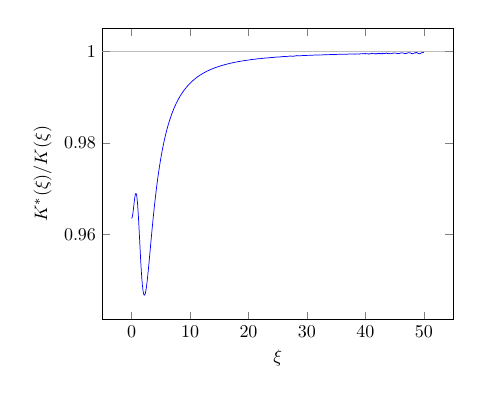
\begin{tikzpicture}[
scale=0.65,]\begin{axis}[
xlabel={$\xi$},
ylabel={$\fdfunc{K}^*(\xi)/\fdfunc{K}(\xi)$},
scaled x ticks = false,
x tick label style = {/pgf/number format/fixed},
scaled y ticks = false,
y tick label style = {/pgf/number format/fixed},
extra y ticks       = 1,
extra y tick labels = ,
extra y tick style  = { grid = major }
]
\addplot[color=blue,] coordinates {
(0.0000000000, 0.9635604621)
(0.0000500000, 0.9635604621)
(0.0002000000, 0.9635604630)
(0.0004500000, 0.9635604668)
(0.0008000000, 0.9635604771)
(0.0012500000, 0.9635604987)
(0.0018000000, 0.9635605379)
(0.0024500000, 0.9635606026)
(0.0032000000, 0.9635607018)
(0.0040500000, 0.9635608461)
(0.0050000000, 0.9635610473)
(0.0060500000, 0.9635613189)
(0.0072000000, 0.9635616756)
(0.0084500000, 0.9635621335)
(0.0098000000, 0.9635627101)
(0.0112500000, 0.9635634244)
(0.0128000000, 0.9635642967)
(0.0144500000, 0.9635653488)
(0.0162000000, 0.9635666036)
(0.0180500000, 0.9635680857)
(0.0200000000, 0.9635698210)
(0.0220500000, 0.9635718365)
(0.0242000000, 0.9635741609)
(0.0264500000, 0.9635768240)
(0.0288000000, 0.9635798571)
(0.0312500000, 0.9635832926)
(0.0338000000, 0.9635871645)
(0.0364500000, 0.9635915077)
(0.0392000000, 0.9635963585)
(0.0420500000, 0.9636017546)
(0.0450000000, 0.9636077348)
(0.0480500000, 0.9636143388)
(0.0512000000, 0.9636216078)
(0.0544500000, 0.9636295838)
(0.0578000000, 0.9636383102)
(0.0612500000, 0.9636478310)
(0.0648000000, 0.9636581914)
(0.0684500000, 0.9636694375)
(0.0722000000, 0.9636816162)
(0.0760500000, 0.9636947751)
(0.0800000000, 0.9637089625)
(0.0840500000, 0.9637242275)
(0.0882000000, 0.9637406197)
(0.0924500000, 0.9637581890)
(0.0968000000, 0.9637769859)
(0.1012500000, 0.9637970609)
(0.1058000000, 0.9638184651)
(0.1104500000, 0.9638412492)
(0.1152000000, 0.9638654641)
(0.1200500000, 0.9638911604)
(0.1250000000, 0.9639183885)
(0.1300500000, 0.9639471983)
(0.1352000000, 0.9639776390)
(0.1404500000, 0.9640097591)
(0.1458000000, 0.9640436063)
(0.1512500000, 0.9640792270)
(0.1568000000, 0.9641166665)
(0.1624500000, 0.9641559685)
(0.1682000000, 0.9641971752)
(0.1740500000, 0.9642403269)
(0.1800000000, 0.9642854616)
(0.1860500000, 0.9643326155)
(0.1922000000, 0.9643818218)
(0.1984500000, 0.9644331113)
(0.2048000000, 0.9644865118)
(0.2112500000, 0.9645420478)
(0.2178000000, 0.9645997402)
(0.2244500000, 0.9646596065)
(0.2312000000, 0.9647216599)
(0.2380500000, 0.9647859096)
(0.2450000000, 0.9648523601)
(0.2520500000, 0.9649210112)
(0.2592000000, 0.9649918576)
(0.2664500000, 0.9650648886)
(0.2738000000, 0.9651400878)
(0.2812500000, 0.9652174331)
(0.2888000000, 0.9652968959)
(0.2964500000, 0.9653784414)
(0.3042000000, 0.9654620277)
(0.3120500000, 0.9655476061)
(0.3200000000, 0.9656351204)
(0.3280500000, 0.9657245070)
(0.3362000000, 0.9658156942)
(0.3444500000, 0.9659086024)
(0.3528000000, 0.9660031435)
(0.3612500000, 0.9660992209)
(0.3698000000, 0.9661967292)
(0.3784500000, 0.9662955538)
(0.3872000000, 0.9663955711)
(0.3960500000, 0.9664966480)
(0.4050000000, 0.9665986420)
(0.4140500000, 0.9667014009)
(0.4232000000, 0.9668047625)
(0.4324500000, 0.9669085551)
(0.4418000000, 0.9670125969)
(0.4512500000, 0.9671166960)
(0.4608000000, 0.9672206507)
(0.4704500000, 0.9673242495)
(0.4802000000, 0.9674272709)
(0.4900500000, 0.9675294835)
(0.5000000000, 0.9676306465)
(0.5100500000, 0.9677305095)
(0.5202000000, 0.9678288129)
(0.5304500000, 0.9679252881)
(0.5408000000, 0.9680196579)
(0.5512500000, 0.9681116364)
(0.5618000000, 0.9682009302)
(0.5724500000, 0.9682872379)
(0.5832000000, 0.9683702514)
(0.5940500000, 0.9684496557)
(0.6050000000, 0.9685251300)
(0.6160500000, 0.9685963482)
(0.6272000000, 0.9686629792)
(0.6384500000, 0.9687246882)
(0.6498000000, 0.9687811371)
(0.6612500000, 0.9688319852)
(0.6728000000, 0.9688768903)
(0.6844500000, 0.9689155096)
(0.6962000000, 0.9689475005)
(0.7080500000, 0.9689725215)
(0.7200000000, 0.9689902334)
(0.7320500000, 0.9690003004)
(0.7442000000, 0.9690023909)
(0.7564500000, 0.9689961790)
(0.7688000000, 0.9689813453)
(0.7812500000, 0.9689575782)
(0.7938000000, 0.9689245751)
(0.8064500000, 0.9688820437)
(0.8192000000, 0.9688297032)
(0.8320500000, 0.9687672852)
(0.8450000000, 0.9686945354)
(0.8580500000, 0.9686112146)
(0.8712000000, 0.9685170999)
(0.8844500000, 0.9684119859)
(0.8978000000, 0.9682956860)
(0.9112500000, 0.9681680336)
(0.9248000000, 0.9680288829)
(0.9384500000, 0.9678781107)
(0.9522000000, 0.9677156163)
(0.9660500000, 0.9675413237)
(0.9800000000, 0.9673551820)
(0.9940500000, 0.9671571663)
(1.0082000000, 0.9669472785)
(1.0224500000, 0.9667255482)
(1.0368000000, 0.9664920333)
(1.0512500000, 0.9662468207)
(1.0658000000, 0.9659900264)
(1.0804500000, 0.9657217965)
(1.0952000000, 0.9654423071)
(1.1100500000, 0.9651517647)
(1.1250000000, 0.9648504060)
(1.1400500000, 0.9645384987)
(1.1552000000, 0.9642163402)
(1.1704500000, 0.9638842582)
(1.1858000000, 0.9635426103)
(1.2012500000, 0.9631917832)
(1.2168000000, 0.9628321923)
(1.2324500000, 0.9624642810)
(1.2482000000, 0.9620885199)
(1.2640500000, 0.9617054059)
(1.2800000000, 0.9613154609)
(1.2960500000, 0.9609192312)
(1.3122000000, 0.9605172854)
(1.3284500000, 0.9601102140)
(1.3448000000, 0.9596986269)
(1.3612500000, 0.9592831528)
(1.3778000000, 0.9588644369)
(1.3944500000, 0.9584431395)
(1.4112000000, 0.9580199340)
(1.4280500000, 0.9575955053)
(1.4450000000, 0.9571705475)
(1.4620500000, 0.9567457621)
(1.4792000000, 0.9563218561)
(1.4964500000, 0.9558995396)
(1.5138000000, 0.9554795242)
(1.5312500000, 0.9550625206)
(1.5488000000, 0.9546492364)
(1.5664500000, 0.9542403743)
(1.5842000000, 0.9538366300)
(1.6020500000, 0.9534386898)
(1.6200000000, 0.9530472291)
(1.6380500000, 0.9526629100)
(1.6562000000, 0.9522863797)
(1.6744500000, 0.9519182685)
(1.6928000000, 0.9515591880)
(1.7112500000, 0.9512097297)
(1.7298000000, 0.9508704628)
(1.7484500000, 0.9505419333)
(1.7672000000, 0.9502246624)
(1.7860500000, 0.9499191451)
(1.8050000000, 0.9496258490)
(1.8240500000, 0.9493452135)
(1.8432000000, 0.9490776485)
(1.8624500000, 0.9488235338)
(1.8818000000, 0.9485832185)
(1.9012500000, 0.9483570202)
(1.9208000000, 0.9481452246)
(1.9404500000, 0.9479480854)
(1.9602000000, 0.9477658240)
(1.9800500000, 0.9475986293)
(2.0000000000, 0.9474466581)
(2.0200500000, 0.9473100350)
(2.0402000000, 0.9471888530)
(2.0604500000, 0.9470831735)
(2.0808000000, 0.9469930273)
(2.1012500000, 0.9469184150)
(2.1218000000, 0.9468593077)
(2.1424500000, 0.9468156481)
(2.1632000000, 0.9467873509)
(2.1840500000, 0.9467743046)
(2.2050000000, 0.9467763715)
(2.2260500000, 0.9467933898)
(2.2472000000, 0.9468251742)
(2.2684500000, 0.9468715174)
(2.2898000000, 0.9469321911)
(2.3112500000, 0.9470069476)
(2.3328000000, 0.9470955209)
(2.3544500000, 0.9471976281)
(2.3762000000, 0.9473129708)
(2.3980500000, 0.9474412364)
(2.4200000000, 0.9475820995)
(2.4420500000, 0.9477352231)
(2.4642000000, 0.9479002600)
(2.4864500000, 0.9480768542)
(2.5088000000, 0.9482646420)
(2.5312500000, 0.9484632535)
(2.5538000000, 0.9486723132)
(2.5764500000, 0.9488914421)
(2.5992000000, 0.9491202581)
(2.6220500000, 0.9493583770)
(2.6450000000, 0.9496054142)
(2.6680500000, 0.9498609852)
(2.6912000000, 0.9501247065)
(2.7144500000, 0.9503961965)
(2.7378000000, 0.9506750765)
(2.7612500000, 0.9509609715)
(2.7848000000, 0.9512535103)
(2.8084500000, 0.9515523270)
(2.8322000000, 0.9518570609)
(2.8560500000, 0.9521673575)
(2.8800000000, 0.9524828688)
(2.9040500000, 0.9528032535)
(2.9282000000, 0.9531281779)
(2.9524500000, 0.9534573158)
(2.9768000000, 0.9537903489)
(3.0012500000, 0.9541269674)
(3.0258000000, 0.9544668694)
(3.0504500000, 0.9548097750)
(3.0752000000, 0.9551553608)
(3.1000500000, 0.9555033902)
(3.1250000000, 0.9558535834)
(3.1500500000, 0.9562056826)
(3.1752000000, 0.9565594387)
(3.2004500000, 0.9569146116)
(3.2258000000, 0.9572709699)
(3.2512500000, 0.9576282910)
(3.2768000000, 0.9579863607)
(3.3024500000, 0.9583449737)
(3.3282000000, 0.9587039328)
(3.3540500000, 0.9590630491)
(3.3800000000, 0.9594221420)
(3.4060500000, 0.9597810387)
(3.4322000000, 0.9601395742)
(3.4584500000, 0.9604975910)
(3.4848000000, 0.9608549392)
(3.5112500000, 0.9612114760)
(3.5378000000, 0.9615670657)
(3.5644500000, 0.9619215794)
(3.5912000000, 0.9622748949)
(3.6180500000, 0.9626268963)
(3.6450000000, 0.9629774741)
(3.6720500000, 0.9633265247)
(3.6992000000, 0.9636739506)
(3.7264500000, 0.9640196596)
(3.7538000000, 0.9643635651)
(3.7812500000, 0.9647055859)
(3.8088000000, 0.9650456457)
(3.8364500000, 0.9653836731)
(3.8642000000, 0.9657196014)
(3.8920500000, 0.9660533686)
(3.9200000000, 0.9663849168)
(3.9480500000, 0.9667141923)
(3.9762000000, 0.9670411457)
(4.0044500000, 0.9673657311)
(4.0328000000, 0.9676879064)
(4.0612500000, 0.9680076331)
(4.0898000000, 0.9683248760)
(4.1184500000, 0.9686396032)
(4.1472000000, 0.9689517859)
(4.1760500000, 0.9692613982)
(4.2050000000, 0.9695684170)
(4.2340500000, 0.9698728221)
(4.2632000000, 0.9701745955)
(4.2924500000, 0.9704737221)
(4.3218000000, 0.9707701888)
(4.3512500000, 0.9710639848)
(4.3808000000, 0.9713551016)
(4.4104500000, 0.9716435324)
(4.4402000000, 0.9719292726)
(4.4700500000, 0.9722123192)
(4.5000000000, 0.9724926712)
(4.5300500000, 0.9727703288)
(4.5602000000, 0.9730452942)
(4.5904500000, 0.9733175707)
(4.6208000000, 0.9735871632)
(4.6512500000, 0.9738540779)
(4.6818000000, 0.9741183221)
(4.7124500000, 0.9743799043)
(4.7432000000, 0.9746388342)
(4.7740500000, 0.9748951224)
(4.8050000000, 0.9751487805)
(4.8360500000, 0.9753998210)
(4.8672000000, 0.9756482573)
(4.8984500000, 0.9758941036)
(4.9298000000, 0.9761373747)
(4.9612500000, 0.9763780861)
(4.9928000000, 0.9766162543)
(5.0244500000, 0.9768518958)
(5.0562000000, 0.9770850281)
(5.0880500000, 0.9773156691)
(5.1200000000, 0.9775438371)
(5.1520500000, 0.9777695508)
(5.1842000000, 0.9779928294)
(5.2164500000, 0.9782136924)
(5.2488000000, 0.9784321597)
(5.2812500000, 0.9786482513)
(5.3138000000, 0.9788619877)
(5.3464500000, 0.9790733895)
(5.3792000000, 0.9792824776)
(5.4120500000, 0.9794892729)
(5.4450000000, 0.9796937966)
(5.4780500000, 0.9798960701)
(5.5112000000, 0.9800961147)
(5.5444500000, 0.9802939520)
(5.5778000000, 0.9804896036)
(5.6112500000, 0.9806830910)
(5.6448000000, 0.9808744360)
(5.6784500000, 0.9810636603)
(5.7122000000, 0.9812507856)
(5.7460500000, 0.9814358336)
(5.7800000000, 0.9816188258)
(5.8140500000, 0.9817997840)
(5.8482000000, 0.9819787298)
(5.8824500000, 0.9821556846)
(5.9168000000, 0.9823306699)
(5.9512500000, 0.9825037071)
(5.9858000000, 0.9826748174)
(6.0204500000, 0.9828440220)
(6.0552000000, 0.9830113419)
(6.0900500000, 0.9831767982)
(6.1250000000, 0.9833404117)
(6.1600500000, 0.9835022029)
(6.1952000000, 0.9836621926)
(6.2304500000, 0.9838204011)
(6.2658000000, 0.9839768487)
(6.3012500000, 0.9841315555)
(6.3368000000, 0.9842845414)
(6.3724500000, 0.9844358264)
(6.4082000000, 0.9845854300)
(6.4440500000, 0.9847333717)
(6.4800000000, 0.9848796708)
(6.5160500000, 0.9850243465)
(6.5522000000, 0.9851674177)
(6.5884500000, 0.9853089032)
(6.6248000000, 0.9854488216)
(6.6612500000, 0.9855871914)
(6.6978000000, 0.9857240308)
(6.7344500000, 0.9858593578)
(6.7712000000, 0.9859931903)
(6.8080500000, 0.9861255462)
(6.8450000000, 0.9862564427)
(6.8820500000, 0.9863858974)
(6.9192000000, 0.9865139273)
(6.9564500000, 0.9866405494)
(6.9938000000, 0.9867657805)
(7.0312500000, 0.9868896372)
(7.0688000000, 0.9870121358)
(7.1064500000, 0.9871332927)
(7.1442000000, 0.9872531238)
(7.1820500000, 0.9873716450)
(7.2200000000, 0.9874888720)
(7.2580500000, 0.9876048202)
(7.2962000000, 0.9877195051)
(7.3344500000, 0.9878329417)
(7.3728000000, 0.9879451451)
(7.4112500000, 0.9880561299)
(7.4498000000, 0.9881659108)
(7.4884500000, 0.9882745022)
(7.5272000000, 0.9883819184)
(7.5660500000, 0.9884881735)
(7.6050000000, 0.9885932814)
(7.6440500000, 0.9886972559)
(7.6832000000, 0.9888001104)
(7.7224500000, 0.9889018585)
(7.7618000000, 0.9890025135)
(7.8012500000, 0.9891020883)
(7.8408000000, 0.9892005959)
(7.8804500000, 0.9892980491)
(7.9202000000, 0.9893944606)
(7.9600500000, 0.9894898426)
(8.0000000000, 0.9895842077)
(8.0400500000, 0.9896775678)
(8.0802000000, 0.9897699350)
(8.1204500000, 0.9898613212)
(8.1608000000, 0.9899517380)
(8.2012500000, 0.9900411970)
(8.2418000000, 0.9901297095)
(8.2824500000, 0.9902172869)
(8.3232000000, 0.9903039403)
(8.3640500000, 0.9903896806)
(8.4050000000, 0.9904745188)
(8.4460500000, 0.9905584654)
(8.4872000000, 0.9906415310)
(8.5284500000, 0.9907237262)
(8.5698000000, 0.9908050611)
(8.6112500000, 0.9908855460)
(8.6528000000, 0.9909651909)
(8.6944500000, 0.9910440057)
(8.7362000000, 0.9911220003)
(8.7780500000, 0.9911991842)
(8.8200000000, 0.9912755670)
(8.8620500000, 0.9913511582)
(8.9042000000, 0.9914259670)
(8.9464500000, 0.9915000027)
(8.9888000000, 0.9915732742)
(9.0312500000, 0.9916457906)
(9.0738000000, 0.9917175607)
(9.1164500000, 0.9917885932)
(9.1592000000, 0.9918588967)
(9.2020500000, 0.9919284797)
(9.2450000000, 0.9919973507)
(9.2880500000, 0.9920655179)
(9.3312000000, 0.9921329895)
(9.3744500000, 0.9921997736)
(9.4178000000, 0.9922658782)
(9.4612500000, 0.9923313111)
(9.5048000000, 0.9923960802)
(9.5484500000, 0.9924601931)
(9.5922000000, 0.9925236574)
(9.6360500000, 0.9925864805)
(9.6800000000, 0.9926486700)
(9.7240500000, 0.9927102330)
(9.7682000000, 0.9927711768)
(9.8124500000, 0.9928315086)
(9.8568000000, 0.9928912352)
(9.9012500000, 0.9929503638)
(9.9458000000, 0.9930089010)
(9.9904500000, 0.9930668538)
(10.0352000000, 0.9931242287)
(10.0800500000, 0.9931810324)
(10.1250000000, 0.9932372713)
(10.1700500000, 0.9932929520)
(10.2152000000, 0.9933480807)
(10.2604500000, 0.9934026637)
(10.3058000000, 0.9934567073)
(10.3512500000, 0.9935102175)
(10.3968000000, 0.9935632004)
(10.4424500000, 0.9936156619)
(10.4882000000, 0.9936676080)
(10.5340500000, 0.9937190444)
(10.5800000000, 0.9937699769)
(10.6260500000, 0.9938204111)
(10.6722000000, 0.9938703527)
(10.7184500000, 0.9939198072)
(10.7648000000, 0.9939687800)
(10.8112500000, 0.9940172766)
(10.8578000000, 0.9940653023)
(10.9044500000, 0.9941128623)
(10.9512000000, 0.9941599618)
(10.9980500000, 0.9942066059)
(11.0450000000, 0.9942527999)
(11.0920500000, 0.9942985485)
(11.1392000000, 0.9943438568)
(11.1864500000, 0.9943887297)
(11.2338000000, 0.9944331720)
(11.2812500000, 0.9944771884)
(11.3288000000, 0.9945207837)
(11.3764500000, 0.9945639624)
(11.4242000000, 0.9946067293)
(11.4720500000, 0.9946490888)
(11.5200000000, 0.9946910454)
(11.5680500000, 0.9947326035)
(11.6162000000, 0.9947737676)
(11.6644500000, 0.9948145418)
(11.7128000000, 0.9948549305)
(11.7612500000, 0.9948949379)
(11.8098000000, 0.9949345682)
(11.8584500000, 0.9949738254)
(11.9072000000, 0.9950127136)
(11.9560500000, 0.9950512369)
(12.0050000000, 0.9950893992)
(12.0540500000, 0.9951272043)
(12.1032000000, 0.9951646563)
(12.1524500000, 0.9952017588)
(12.2018000000, 0.9952385158)
(12.2512500000, 0.9952749334)
(12.3008000000, 0.9953110075)
(12.3504500000, 0.9953467497)
(12.4002000000, 0.9953821609)
(12.4500500000, 0.9954172446)
(12.5000000000, 0.9954520045)
(12.5500500000, 0.9954864438)
(12.6002000000, 0.9955205662)
(12.6504500000, 0.9955543748)
(12.7008000000, 0.9955878732)
(12.7512500000, 0.9956210646)
(12.8018000000, 0.9956539426)
(12.8524500000, 0.9956865225)
(12.9032000000, 0.9957188292)
(12.9540500000, 0.9957508248)
(13.0050000000, 0.9957825294)
(13.0560500000, 0.9958139460)
(13.1072000000, 0.9958450776)
(13.1584500000, 0.9958759273)
(13.2098000000, 0.9959064980)
(13.2612500000, 0.9959367927)
(13.3128000000, 0.9959668142)
(13.3644500000, 0.9959966032)
(13.4162000000, 0.9960261028)
(13.4680500000, 0.9960553342)
(13.5200000000, 0.9960842257)
(13.5720500000, 0.9961129237)
(13.6242000000, 0.9961413653)
(13.6764500000, 0.9961695532)
(13.7288000000, 0.9961974898)
(13.7812500000, 0.9962251779)
(13.8338000000, 0.9962526201)
(13.8864500000, 0.9962798188)
(13.9392000000, 0.9963067765)
(13.9920500000, 0.9963333515)
(14.0450000000, 0.9963599793)
(14.0980500000, 0.9963862291)
(14.1512000000, 0.9964122478)
(14.2044500000, 0.9964380377)
(14.2578000000, 0.9964636012)
(14.3112500000, 0.9964889406)
(14.3648000000, 0.9965140582)
(14.4184500000, 0.9965389562)
(14.4722000000, 0.9965636369)
(14.5260500000, 0.9965881025)
(14.5800000000, 0.9966123552)
(14.6340500000, 0.9966363972)
(14.6882000000, 0.9966602305)
(14.7424500000, 0.9966838574)
(14.7968000000, 0.9967072798)
(14.8512500000, 0.9967304999)
(14.9058000000, 0.9967535197)
(14.9604500000, 0.9967763413)
(15.0152000000, 0.9967989665)
(15.0700500000, 0.9968213974)
(15.1250000000, 0.9968436360)
(15.1800500000, 0.9968656842)
(15.2352000000, 0.9968875438)
(15.2904500000, 0.9969092168)
(15.3458000000, 0.9969307050)
(15.4012500000, 0.9969520102)
(15.4568000000, 0.9969731344)
(15.5124500000, 0.9969940792)
(15.5682000000, 0.9970148465)
(15.6240500000, 0.9970354381)
(15.6800000000, 0.9970558556)
(15.7360500000, 0.9970761008)
(15.7922000000, 0.9970961754)
(15.8484500000, 0.9971160811)
(15.9048000000, 0.9971358195)
(15.9612500000, 0.9971553923)
(16.0178000000, 0.9971748012)
(16.0744500000, 0.9971940477)
(16.1312000000, 0.9972131333)
(16.1880500000, 0.9972320598)
(16.2450000000, 0.9972508287)
(16.3020500000, 0.9972694414)
(16.3592000000, 0.9972878995)
(16.4164500000, 0.9973062046)
(16.4738000000, 0.9973243580)
(16.5312500000, 0.9973423613)
(16.5888000000, 0.9973602160)
(16.6464500000, 0.9973779235)
(16.7042000000, 0.9973954851)
(16.7620500000, 0.9974129023)
(16.8200000000, 0.9974301766)
(16.8780500000, 0.9974473092)
(16.9362000000, 0.9974643016)
(16.9944500000, 0.9974811550)
(17.0528000000, 0.9974978709)
(17.1112500000, 0.9975144505)
(17.1698000000, 0.9975308951)
(17.2284500000, 0.9975472061)
(17.2872000000, 0.9975633847)
(17.3460500000, 0.9975794322)
(17.4050000000, 0.9975953498)
(17.4640500000, 0.9976161258)
(17.5232000000, 0.9976268003)
(17.5824500000, 0.9976423356)
(17.6418000000, 0.9976577459)
(17.7012500000, 0.9976730323)
(17.7608000000, 0.9976881961)
(17.8204500000, 0.9977032384)
(17.8802000000, 0.9977181603)
(17.9400500000, 0.9977264801)
(18.0000000000, 0.9977405475)
(18.0600500000, 0.9977554775)
(18.1202000000, 0.9977766669)
(18.1804500000, 0.9977910037)
(18.2408000000, 0.9978052268)
(18.3012500000, 0.9978193372)
(18.3618000000, 0.9978333360)
(18.4224500000, 0.9978472242)
(18.4832000000, 0.9978610028)
(18.5440500000, 0.9978746729)
(18.6050000000, 0.9978882354)
(18.6660500000, 0.9979070390)
(18.7272000000, 0.9979168728)
(18.7884500000, 0.9979282876)
(18.8498000000, 0.9979414298)
(18.9112500000, 0.9979544694)
(18.9728000000, 0.9979674072)
(19.0344500000, 0.9979802440)
(19.0962000000, 0.9979820774)
(19.1580500000, 0.9979975383)
(19.2200000000, 0.9980142409)
(19.2820500000, 0.9980316513)
(19.3442000000, 0.9980429496)
(19.4064500000, 0.9980552010)
(19.4688000000, 0.9980673579)
(19.5312500000, 0.9980794212)
(19.5938000000, 0.9980913916)
(19.6564500000, 0.9981145582)
(19.7192000000, 0.9981215856)
(19.7820500000, 0.9981273274)
(19.8450000000, 0.9981326018)
(19.9080500000, 0.9981383244)
(19.9712000000, 0.9981453774)
(20.0344500000, 0.9981726558)
(20.0978000000, 0.9981839128)
(20.1612500000, 0.9981950855)
(20.2248000000, 0.9982061717)
(20.2884500000, 0.9982171761)
(20.3522000000, 0.9982330761)
(20.4160500000, 0.9982511556)
(20.4800000000, 0.9982676634)
(20.5440500000, 0.9982816825)
(20.6082000000, 0.9982709586)
(20.6724500000, 0.9982814747)
(20.7368000000, 0.9982919110)
(20.8012500000, 0.9983022688)
(20.8658000000, 0.9983087026)
(20.9304500000, 0.9983101305)
(20.9952000000, 0.9983130118)
(21.0600500000, 0.9983184869)
(21.1250000000, 0.9983273430)
(21.1900500000, 0.9983398818)
(21.2552000000, 0.9983726357)
(21.3204500000, 0.9983823917)
(21.3858000000, 0.9983920759)
(21.4512500000, 0.9984016890)
(21.5168000000, 0.9984328727)
(21.5824500000, 0.9984482431)
(21.6482000000, 0.9984596315)
(21.7140500000, 0.9984394379)
(21.7800000000, 0.9984693610)
(21.8460500000, 0.9984579016)
(21.9122000000, 0.9984670300)
(21.9784500000, 0.9984760910)
(22.0448000000, 0.9984850853)
(22.1112500000, 0.9984633808)
(22.1778000000, 0.9984693654)
(22.2444500000, 0.9984802438)
(22.3112000000, 0.9984958599)
(22.3780500000, 0.9985153241)
(22.4450000000, 0.9985376994)
(22.5120500000, 0.9985462440)
(22.5792000000, 0.9985547323)
(22.6464500000, 0.9985631597)
(22.7138000000, 0.9985715231)
(22.7812500000, 0.9986154904)
(22.8488000000, 0.9986164117)
(22.9164500000, 0.9986127641)
(22.9842000000, 0.9986062254)
(23.0520500000, 0.9986124551)
(23.1200000000, 0.9986204630)
(23.1880500000, 0.9986284135)
(23.2562000000, 0.9986363134)
(23.3244500000, 0.9986441541)
(23.3928000000, 0.9986200692)
(23.4612500000, 0.9986407902)
(23.5298000000, 0.9986646746)
(23.5984500000, 0.9986893089)
(23.6672000000, 0.9986825343)
(23.7360500000, 0.9986900507)
(23.8050000000, 0.9986975127)
(23.8740500000, 0.9987049110)
(23.9432000000, 0.9987122663)
(24.0124500000, 0.9987402396)
(24.0818000000, 0.9987296477)
(24.1512500000, 0.9987181711)
(24.2208000000, 0.9987086978)
(24.2904500000, 0.9987482622)
(24.3602000000, 0.9987553149)
(24.4300500000, 0.9987623305)
(24.5000000000, 0.9987692842)
(24.5700500000, 0.9987545408)
(24.6402000000, 0.9987809798)
(24.7104500000, 0.9988080913)
(24.7808000000, 0.9988327003)
(24.8512500000, 0.9988033579)
(24.9218000000, 0.9988100181)
(24.9924500000, 0.9988166272)
(25.0632000000, 0.9988232057)
(25.1340500000, 0.9988512964)
(25.2050000000, 0.9988363686)
(25.2760500000, 0.9988209781)
(25.3472000000, 0.9988085840)
(25.4184500000, 0.9988022349)
(25.4898000000, 0.9988617345)
(25.5612500000, 0.9988680347)
(25.6328000000, 0.9988742286)
(25.7044500000, 0.9988804119)
(25.7762000000, 0.9988897476)
(25.8480500000, 0.9989190385)
(25.9200000000, 0.9989444450)
(25.9920500000, 0.9989627877)
(26.0642000000, 0.9989106544)
(26.1364500000, 0.9989165329)
(26.2088000000, 0.9989223840)
(26.2812500000, 0.9989283921)
(26.3538000000, 0.9989260400)
(26.4264500000, 0.9989075668)
(26.4992000000, 0.9988939415)
(26.5720500000, 0.9988883942)
(26.6450000000, 0.9989572605)
(26.7180500000, 0.9989629674)
(26.7912000000, 0.9989685960)
(26.8644500000, 0.9989738473)
(26.9378000000, 0.9989943075)
(27.0112500000, 0.9990246212)
(27.0848000000, 0.9990487175)
(27.1584500000, 0.9990634326)
(27.2322000000, 0.9990006285)
(27.3060500000, 0.9990058806)
(27.3800000000, 0.9990111905)
(27.4540500000, 0.9990216125)
(27.5282000000, 0.9989985636)
(27.6024500000, 0.9989790283)
(27.6768000000, 0.9989671679)
(27.7512500000, 0.9989659256)
(27.8258000000, 0.9990435216)
(27.9004500000, 0.9990485654)
(27.9752000000, 0.9990534066)
(28.0500500000, 0.9990627934)
(28.1250000000, 0.9990967652)
(28.2000500000, 0.9991253375)
(28.2752000000, 0.9990715477)
(28.3504500000, 0.9990761906)
(28.4258000000, 0.9990810416)
(28.5012500000, 0.9990861288)
(28.5768000000, 0.9990918346)
(28.6524500000, 0.9990795118)
(28.7282000000, 0.9990554414)
(28.8040500000, 0.9991059539)
(28.8800000000, 0.9991125029)
(28.9560500000, 0.9991170646)
(29.0322000000, 0.9991211860)
(29.1084500000, 0.9991243586)
(29.1848000000, 0.9991288860)
(29.2612500000, 0.9991333843)
(29.3378000000, 0.9991378537)
(29.4144500000, 0.9991422944)
(29.4912000000, 0.9991467068)
(29.5680500000, 0.9991510911)
(29.6450000000, 0.9991554476)
(29.7220500000, 0.9991597764)
(29.7992000000, 0.9991640777)
(29.8764500000, 0.9991683516)
(29.9538000000, 0.9991725982)
(30.0312500000, 0.9991768179)
(30.1088000000, 0.9991810107)
(30.1864500000, 0.9991851770)
(30.2642000000, 0.9991893170)
(30.3420500000, 0.9991934311)
(30.4200000000, 0.9991975195)
(30.4980500000, 0.9992015822)
(30.5762000000, 0.9992056194)
(30.6544500000, 0.9992096312)
(30.7328000000, 0.9992136175)
(30.8112500000, 0.9992175787)
(30.8898000000, 0.9992215151)
(30.9684500000, 0.9992254268)
(31.0472000000, 0.9992293144)
(31.1260500000, 0.9992331779)
(31.2050000000, 0.9992370177)
(31.2840500000, 0.9992408337)
(31.3632000000, 0.9992446260)
(31.4424500000, 0.9992483944)
(31.5218000000, 0.9992521391)
(31.6012500000, 0.9992558604)
(31.6808000000, 0.9992595586)
(31.7604500000, 0.9992632342)
(31.8402000000, 0.9992668875)
(31.9200500000, 0.9992795468)
(32.0000000000, 0.9992868724)
(32.0800500000, 0.9992843133)
(32.1602000000, 0.9992812795)
(32.2404500000, 0.9992848218)
(32.3208000000, 0.9992883419)
(32.4012500000, 0.9992842029)
(32.4818000000, 0.9992814509)
(32.5624500000, 0.9992814587)
(32.6432000000, 0.9992838183)
(32.7240500000, 0.9993056253)
(32.8050000000, 0.9993090202)
(32.8860500000, 0.9993123942)
(32.9672000000, 0.9993157471)
(33.0484500000, 0.9993190789)
(33.1298000000, 0.9993223901)
(33.2112500000, 0.9993546237)
(33.2928000000, 0.9993177485)
(33.3744500000, 0.9993322062)
(33.4562000000, 0.9993354404)
(33.5380500000, 0.9993386555)
(33.6200000000, 0.9993418510)
(33.7020500000, 0.9993450265)
(33.7842000000, 0.9993291524)
(33.8664500000, 0.9993545754)
(33.9488000000, 0.9993544346)
(34.0312500000, 0.9993575335)
(34.1138000000, 0.9993606150)
(34.1964500000, 0.9993636793)
(34.2792000000, 0.9993667259)
(34.3620500000, 0.9993697542)
(34.4450000000, 0.9993747849)
(34.5280500000, 0.9993348342)
(34.6112000000, 0.9993787248)
(34.6944500000, 0.9993816781)
(34.7778000000, 0.9993846147)
(34.8612500000, 0.9993875354)
(34.9448000000, 0.9993904403)
(35.0284500000, 0.9993891008)
(35.1122000000, 0.9993962004)
(35.1960500000, 0.9993990538)
(35.2800000000, 0.9994018887)
(35.3640500000, 0.9994047055)
(35.4482000000, 0.9994075054)
(35.5324500000, 0.9994102897)
(35.6168000000, 0.9994130597)
(35.7012500000, 0.9994158149)
(35.7858000000, 0.9994185554)
(35.8704500000, 0.9994212797)
(35.9552000000, 0.9993977791)
(36.0400500000, 0.9994226380)
(36.1250000000, 0.9994293473)
(36.2100500000, 0.9994320034)
(36.2952000000, 0.9994346447)
(36.3804500000, 0.9994372729)
(36.4658000000, 0.9994398881)
(36.5512500000, 0.9994424895)
(36.6368000000, 0.9994330546)
(36.7224500000, 0.9994476454)
(36.8082000000, 0.9994531670)
(36.8940500000, 0.9994146075)
(36.9800000000, 0.9994552528)
(37.0660500000, 0.9994577600)
(37.1522000000, 0.9994602553)
(37.2384500000, 0.9994627388)
(37.3248000000, 0.9994652090)
(37.4112500000, 0.9994635447)
(37.4978000000, 0.9994701056)
(37.5844500000, 0.9995064591)
(37.6712000000, 0.9994749358)
(37.7580500000, 0.9994773288)
(37.8450000000, 0.9994797100)
(37.9320500000, 0.9994820806)
(38.0192000000, 0.9994844405)
(38.1064500000, 0.9994497512)
(38.1938000000, 0.9994169735)
(38.2812500000, 0.9995022278)
(38.3688000000, 0.9994937404)
(38.4564500000, 0.9994960280)
(38.5442000000, 0.9994983006)
(38.6320500000, 0.9994986908)
(38.7200000000, 0.9995028178)
(38.8080500000, 0.9995050617)
(38.8962000000, 0.9995072940)
(38.9844500000, 0.9994563796)
(39.0728000000, 0.9995117167)
(39.1612500000, 0.9995139030)
(39.2498000000, 0.9995079084)
(39.3384500000, 0.9995063776)
(39.4272000000, 0.9995406864)
(39.5160500000, 0.9995705353)
(39.6050000000, 0.9995246639)
(39.6940500000, 0.9995267895)
(39.7832000000, 0.9995288988)
(39.8724500000, 0.9995577213)
(39.9618000000, 0.9996094611)
(40.0512500000, 0.9994935598)
(40.1408000000, 0.9995371929)
(40.2304500000, 0.9995392428)
(40.3202000000, 0.9995412820)
(40.4100500000, 0.9995484996)
(40.5000000000, 0.9994935732)
(40.5900500000, 0.9994499507)
(40.6802000000, 0.9995493314)
(40.7704500000, 0.9995513080)
(40.8608000000, 0.9995532711)
(40.9512500000, 0.9995552296)
(41.0418000000, 0.9995813062)
(41.1324500000, 0.9996367610)
(41.2232000000, 0.9996741084)
(41.3140500000, 0.9995629817)
(41.4050000000, 0.9995648904)
(41.4960500000, 0.9995134643)
(41.5872000000, 0.9995717666)
(41.6784500000, 0.9995885310)
(41.7698000000, 0.9994752556)
(41.8612500000, 0.9994567764)
(41.9528000000, 0.9995761101)
(42.0444500000, 0.9995779526)
(42.1362000000, 0.9995525307)
(42.2280500000, 0.9996097588)
(42.3200000000, 0.9996591804)
(42.4120500000, 0.9995851907)
(42.5042000000, 0.9995072212)
(42.5964500000, 0.9995887522)
(42.6888000000, 0.9996370896)
(42.7812500000, 0.9995886605)
(42.8738000000, 0.9996342043)
(42.9664500000, 0.9995101518)
(43.0592000000, 0.9995975158)
(43.1520500000, 0.9996723021)
(43.2450000000, 0.9996009380)
(43.3380500000, 0.9995842426)
(43.4312000000, 0.9996301418)
(43.5244500000, 0.9996683845)
(43.6178000000, 0.9996911763)
(43.7112500000, 0.9996093812)
(43.8048000000, 0.9996110390)
(43.8984500000, 0.9996497154)
(43.9922000000, 0.9996135723)
(44.0860500000, 0.9995792414)
(44.1800000000, 0.9995542887)
(44.2740500000, 0.9995438547)
(44.3682000000, 0.9995497597)
(44.4624500000, 0.9995703674)
(44.5568000000, 0.9996011533)
(44.6512500000, 0.9996357873)
(44.7458000000, 0.9996674688)
(44.8404500000, 0.9996902406)
(44.9352000000, 0.9997000587)
(45.0300500000, 0.9996954617)
(45.1250000000, 0.9996777704)
(45.2200500000, 0.9996508148)
(45.3152000000, 0.9996202440)
(45.4104500000, 0.9995925201)
(45.5058000000, 0.9995737347)
(45.6012500000, 0.9995684229)
(45.6968000000, 0.9995785751)
(45.7924500000, 0.9996030528)
(45.8882000000, 0.9996375758)
(45.9840500000, 0.9996753704)
(46.0800000000, 0.9997084368)
(46.1760500000, 0.9997292424)
(46.2722000000, 0.9997325068)
(46.3684500000, 0.9997166619)
(46.4648000000, 0.9996845799)
(46.5612500000, 0.9996432898)
(46.6578000000, 0.9996026215)
(46.7544500000, 0.9995729986)
(46.8512000000, 0.9995628536)
(46.9480500000, 0.9995763063)
(47.0450000000, 0.9996117496)
(47.1420500000, 0.9996618134)
(47.2392000000, 0.9997148509)
(47.3364500000, 0.9997576874)
(47.4338000000, 0.9997789964)
(47.5312500000, 0.9997724350)
(47.6288000000, 0.9997386623)
(47.7264500000, 0.9996855992)
(47.8242000000, 0.9996267311)
(47.9220500000, 0.9995777839)
(48.0200000000, 0.9995525865)
(48.1180500000, 0.9995592156)
(48.2162000000, 0.9995975100)
(48.3144500000, 0.9996587251)
(48.4128000000, 0.9997275375)
(48.5112500000, 0.9997859628)
(48.6098000000, 0.9996932271)
(48.7084500000, 0.9998149842)
(48.8072000000, 0.9997765273)
(48.9060500000, 0.9997126413)
(49.0050000000, 0.9996404271)
(49.1040500000, 0.9995797632)
(49.2032000000, 0.9995478901)
(49.3024500000, 0.9995545595)
(49.4018000000, 0.9995991238)
(49.5012500000, 0.9996704407)
(49.6008000000, 0.9997497052)
(49.7004500000, 0.9998154970)
(49.8002000000, 0.9998496919)
(49.9000500000, 0.9998425997)
(50.0000000000, 0.9997958614)
};
\end{axis}\end{tikzpicture}
}
    \caption{Comparison of the \idxs{impulse}{response} of \eqref{eq:empirical} and the impulse response of an ideal kernel. The fluctuations for the higher values of $\xi$ in \subrefp{fig:transformedkernelratio} are purely due to \idxs{numerical}{errors} in the solution of \eqref{eq:kerneltofdkernelmodified}.}
    \label{fig:transformedkernel}
\end{figure}

Expanding \eqref{eq:opcfconvolution} yields

\begin{equation} \label{eq:opcfintegral}
\sop{C}\,\eta(\vec{r},\,t) \,=\, \int_{\mathbb{R}^2}f(\Delta\vec{r})\,\eta(\vec{r}-\Delta\vec{r},\,t)\,\opd\Delta\vec{r}
\end{equation}

which, by using \eqref{eq:ftokernel}, can be rewritten to

\begin{equation} \label{eq:opchunknown}
\sop{C}_h\,\eta(\vec{r},\,t) \,=\, a_h\int_{\mathbb{R}^2}K\left(\frac{\Delta\vec{r}}{h}\right)\,\eta(\vec{r}-\Delta\vec{r},\,t)\,\opd\Delta\vec{r},
\end{equation}

where the index $h$ is introduced to make it apparent that $\sop{C}$ is actually a function of the \idxs{water}{depth} $h$, and where

\begin{equation} \label{eq:aofh}
a_h \,=\, 1/h^2.
\end{equation}

We could just use this definition of $\sop{C}$ and plug it into \eqref{eq:diffeqspatial} and, by being \naive and \assuming that since \eqref{eq:diffeqspatial} is independent of $\vec{k}$, it would describe not only the behavior of single wave components fixed to a specific wave vector $\vec{k}$ which are described by \eqref{eq:component}, but the behavior of any free surface elevation $\eta(\vec{r},\,t)$, we would have a \PDE that we could use for simulating single wave components as well as complex (in the sense of being non-simple) surfaces.

A problem, though, is that $h$ is not a constant unless the sea bottom is perfectly flat, but dependent on the location, so \eqref{eq:opchunknown} is not directly applicable. The simplest remedy for this would be to just substitute $h$ for the water depth of the local position $h(\vec{r})$:

\begin{equation} \label{eq:opchlocal}
\sop{C}_{h(\vec{r})}\,\eta(\vec{r},\,t) \,=\, a_{h(\vec{r})}\int_{\mathbb{R}^2}K\left(\frac{\Delta\vec{r}}{h(\vec{r})}\right)\,\eta(\vec{r}-\Delta\vec{r},\,t)\,\opd\Delta\vec{r},
\end{equation}

where $a_{h(\vec{r})} = 1/h^2(\vec{r})$. Unfortunately, this method has other problems that occur when the bottom topography is unpleasant. For example, if one part of the water is surrounded by ground, as is the case with lakes, this simple version of the operator would be affected by parts of the water from which $\vec{r}$ is isolated. Hence, waves in one lake could, similar to in \idxs{quantum}{mechanics}, \tunnel into another, nearby lake, which is not the case in reality.

A possible remedy for this problem is to try to limit the convolution filter and let the kernel approach zero more quickly when the water gets shallower. For example, one could be to find the path from $\vec{r}$ to $\vec{r}-\Delta\vec{r}$ with the maximal minimal water depth, and use the minimal water depth of that path as an \idxs{effective}{water depth} $h_e$ for that sampling location. Another possibility could be to find the path with the minimal path integral of $h^{-1}$, calculate the average value of $h^{-1}$ along that path and use the inverse of that average as the effective depth $h_e$.

%TODO: How is h_e calculated? How much time does that take?

Anyway, assuming we have defined an effective depth \mbox{$h_e(\vec{r},\,\vec{r}-\Delta\vec{r})$} in some way, which can be calculated efficiently (this essentially means in $O(1)$ time in average for any distance $|\Delta\vec{r}\,|$), we can use that definition:

\begin{equation} \label{eq:opcheffective}
\sop{C}_{h_e}\,\eta(\vec{r},\,t) \,=\, a_{h_e}\,\int_{\mathbb{R}^2}K\left(\frac{\Delta\vec{r}}{h_e(\vec{r},\,\vec{r}-\Delta\vec{r})}\right)\,\eta(\vec{r}-\Delta\vec{r},\,t)\,\opd\Delta\vec{r}
\end{equation}

which will be the most general definition of $\sop{C}$ and hopefully robust enough to be useful in a simulation. Here, $a_{h_e}$ is an unknown \idxs{scale}{factor} associated with $h_e$. One problem here, though, is that different values for $h_e$ are used for each value of $\vec{r}$, so there is no trivial way to obtain $a_{h_e}$. However, by examining \eqref{eq:transkernelofxivec}, we see that the convolution filter is in fact a kind of \idxs{low-pass}{filter}, since $\fdfunc{K}(\vec{0}) = 1$. We therefore require that if we apply it on a constant function, it will have no effect:

\begin{equation} \label{eq:opcproperscaling}
\sop{C}\,\eta(\vec{r},\,t) \,=\, \eta(\vec{r},\,t),\quad\eta(\vec{r},\,t) \,=\, \eta_0\ \forall\ \vec{r},\,t.
\end{equation}

By combining \eqref{eq:opcheffective} and \eqref{eq:opcproperscaling} and isolating $a_{h_e}$, we get

\begin{equation} \label{eq:scalingheffective}
a_{h_e} \,=\, \frac{1}{\displaystyle\int_{\mathbb{R}^2}K\left(\frac{\Delta\vec{r}}{h_e(\vec{r},\,\vec{r}-\Delta\vec{r})}\right) \opd\Delta\vec{r}}.
\end{equation}

By using the effective water depth $h_e$, and $\sop{C}_{h_e}$, which is the most \idx{robust} of our $\sop{C}$ operators, \eqref{eq:diffeqspatial} becomes

\begin{equation} \label{eq:diffeqonehstillunknown}
\sop{\omega}^2\,\eta \,=\, h\,\left(g\,+\,\frac{\gamma}{\rho}\,\sop{k^2}\right)\,\sop{k^2}\,\sop{C}_{h_e}\,\eta
\end{equation}

which still contains $h$ at one place. Using \eqref{eq:aofh}, we can substitute $h$ for $a_{h_e}^{-1/2}$ and obtain

\begin{equation} \label{eq:diffeqcomplete}
\sop{\omega}^2\,\eta \,=\, a_{h_e}^{-1/2}\,\left(g\,+\,\frac{\gamma}{\rho}\,\sop{k^2}\right)\,\sop{k^2}\,\sop{C}_{h_e}\,\eta
\end{equation}

which is a \PDE completely free from variables in the frequency domain and which is believed to be robust even for varying water depths, which was the goal. By using the definition for $\sop{\omega}$ (\eqref{eq:opomega}), the definition for $\sop{k^2}$ (\eqref{eq:opk2}) and the definition for $\sop{C}_{h_e}$ (\eqref{eq:opcheffective}, \eqref{eq:scalingheffective}), the equation can be rewritten as

\begin{equation} \label{eq:diffeqnouserdefinedoperators}
\frac{\partial^2}{\partial t^2}\,\eta \,=\, a_{h_e}^{-1/2}\,\left(g\,-\,\frac{\gamma}{\rho}\,\nabla^2\right)\,\nabla^2\,\frac{\displaystyle\int_{\mathbb{R}^2}K\left(\frac{\Delta\vec{r}}{h_e(\vec{r},\,\vec{r}-\Delta\vec{r})}\right)\,\eta(\vec{r}-\Delta\vec{r},\,t)\,\opd\Delta\vec{r}}{\displaystyle\int_{\mathbb{R}^2}K\left(\frac{\Delta\vec{r}}{h_e(\vec{r},\,\vec{r}-\Delta\vec{r})}\right) \opd\Delta\vec{r}}.
\end{equation}

Note that the order of the operators matters when we use this definition for $C$, contrary to in \eqref{eq:dispersion_again} which we started from, where the order of the factors on the right hand side doesn't matter. If, for example, \eqref{eq:diffeqcomplete} is modified so that $C_{h_e}$ is placed furthest to the left, we end up with the \PDE

\begin{equation} \label{eq:diffeqnouserdefinedoperatorsvariant}
\frac{\partial^2}{\partial t^2}\,\eta \,=\, \frac{\displaystyle\int_{\mathbb{R}^2}K\left(\frac{\Delta\vec{r}}{h_e(\vec{r},\,\vec{r}-\Delta\vec{r})}\right)\,\left(g\,-\,\frac{\gamma}{\rho}\,\nabla^2\right)\,\nabla^2\,\eta(\vec{r}-\Delta\vec{r},\,t)\,\opd\Delta\vec{r}}{\sqrt{\displaystyle\int_{\mathbb{R}^2}K\left(\frac{\Delta\vec{r}}{h_e(\vec{r},\,\vec{r}-\Delta\vec{r})}\right) \opd\Delta\vec{r}}}
\end{equation}

instead, which is different from \eqref{eq:diffeqnouserdefinedoperators}. It is unknown which order of the operators would be the most "appropriate".

\section{Applying the convolution filter}

For a \idxs{uniform}{surface grid}, the convolution filter can be applied by using a modified version of the \FMM\index{algorithm!fast multipole method|see{fast multipole method}} \citep{Greengard1985,Greengard1987a} for continuous data, the \CFMM\index{algorithm!continuous fast multipole method|see{continuous fast multipole method}} \citep{White1994}, which allows it to be applied with a $O(N)$\indexs{big O}{notation} \idx{time complexity} instead of $O(N^2)$ as with a simple $N$-to-$N$ approach, where $N$ is the number of surface grid points.

However, even though $O(N)$ is very fast in theory, the \CFMM is complicated and involves many computational steps which would make the simulation slow. It requires a high-order \idxs{Taylor}{polynomial} in order to make a good \approximation, so one would have to balance the approximation errors to the additional computational costs due to the processing of the Taylor polynomial. On the other hand, it is possible to parallelize these kinds of algorithms \citep[see e.g.][]{Board1994}, making it possible to overcome this bottleneck simply by running the algorithm on many \idxp{core}{s}.
